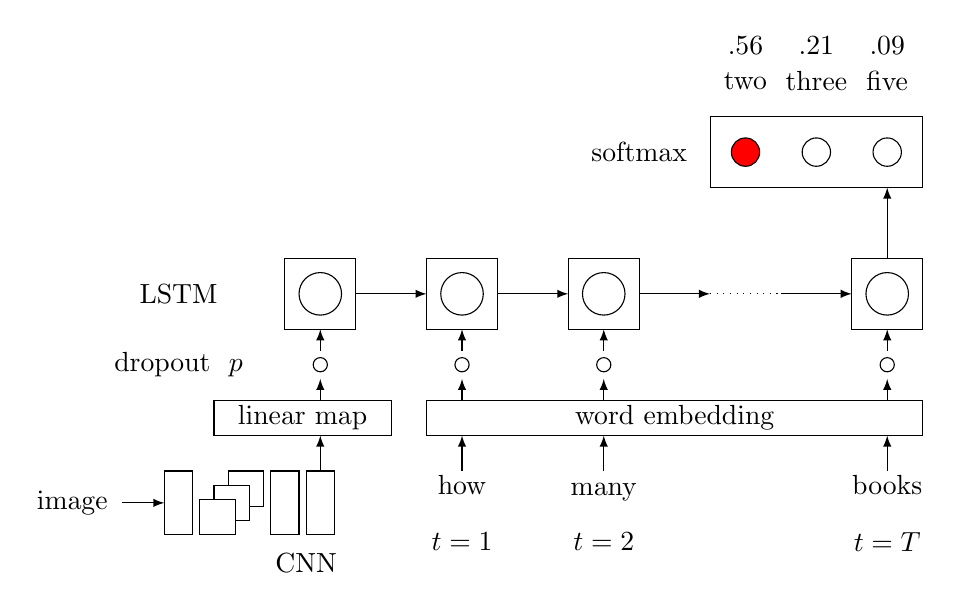
\begin{tikzpicture}[scale=0.9]
\foreach \x in  {5, 7, 9, 13}
{
	\draw (\x,1) rectangle (\x+1,2);
	\draw (\x+0.5,1.5) circle (0.3cm);
	\draw [-latex](\x+0.5,0) -- (\x+0.5,0.3);
	\draw (\x+0.5,0.5) circle (0.1cm);
	\draw [-latex](\x+0.5,0.7) -- (\x+0.5,1);
}

\foreach \x in  {7, 9, 13}
{
	\draw [-latex](\x+0.5,-1) -- (\x+0.5,-0.5);
}

\foreach \x in  {7, 9, 11, 13}
{
	\draw [-latex](\x-1,1.5) -- (\x,1.5);
}

\path (7.5,-2) node[draw=none] (t0) {$t=1$};
\path (9.5,-2) node[draw=none] (t1) {$t=2$};
\path (13.5,-2) node[draw=none] (tT1) {$t=T$};
\draw [dotted] (11,1.5) -- (12,1.5);

\path (7.5,-1.2) node[draw=none] (w1) {how};
\path (9.5,-1.3) node[draw=none] (w2) {many};
\path (13.5,-1.2) node[draw=none] (w3) {books};
\path (3.5,0.5) node[draw=none] (drop) {dropout $~p$};
\path (3.5,1.5) node[draw=none] (lstm1) {LSTM};
\draw (7, -0.5) rectangle (14, 0);

\draw (11,3) rectangle (14,4);
\draw[fill=red] (11.5,3.5) circle (0.2cm);
\draw (12.5,3.5) circle (0.2cm);
\draw (13.5,3.5) circle (0.2cm);
\path (10,3.5) node[draw=none] (logit) {softmax};
\path (11.5,4.5) node[draw=none] (logit2) {two};
\path (12.5,4.5) node[draw=none] (logit3) {three};
\path (13.5,4.5) node[draw=none] (logit5) {five};
\path (11.5,5) node[draw=none] (logit2) {.56};
\path (12.5,5) node[draw=none] (logit3) {.21};
\path (13.5,5) node[draw=none] (logit5) {.09};
\draw [-latex] (13.5,2) -- (13.5,3);

\draw (4,-0.5) rectangle (6.5, 0);
\path (5.25,-0.25) node[draw=none] (imgMap) {linear map};

\draw (3.3, -1.9) rectangle (3.7, -1);
\draw[fill=white] (4.2, -1.5) rectangle (4.7, -1);
\draw[fill=white] (4.0, -1.7) rectangle (4.5, -1.2);
\draw[fill=white] (3.8, -1.9) rectangle (4.3, -1.4);
\draw (4.8, -1.9) rectangle (5.2, -1);
\draw (5.3, -1.9) rectangle (5.7, -1);
\draw [-latex] (5.5, -1.0) -- (5.5, -0.5);

\draw [-latex] (2.7,-1.45) -- (3.3, -1.45);
\path (2.0,-1.45) node[draw=none] (image) {image};
\path (5.3,-2.3) node[draw=none] (cnn) {CNN};
\path (10.5,-0.25) node[draw=none] (Wemb) {word embedding};

\end{tikzpicture}